\chapter{Results}
\label{chap:results}

The results of four simple benchmarks of WARP against Serpent 2.1.18 and MCNP 6.1 are presented in this section.  All of the benchmarks make use nuclear data loaded from the ACE libraries that Serpent uses.  MCNP 6.1 uses the nuclear data distributed with it, which is also from ENDFB/VII, but since the library files are identical between Serpent and WARP, the error comparisons in this section are made against Serpent, not MCNP.  WARP only uses collision estimators for flux tallies and $k_\mathrm{eff}$ estimations, so the collision estimates from Serpent and MCNP are also used.  Serpent and MCNP have more sophisticated estimators as well, but a comparing WARP against their collision estimators specifically will provide the fairest comparison.  Serpent and MCNP are also run serially, which gives them the best theoretical performance when is comes to scaling, i.e. they are assumed to scale perfectly linearly.  In this way, the card that WARP runs on can be equivocated to a certain number of CPU cores, and a conservative performance per cost comparison can be made.

All of the benchmark cases were run on a server containing two AMD Opteron 6128 Magny-Cours processors.  These processors each contain eight cores which are clocked at 2.0Ghz and have a 512kB L2 cache.  The server has 32 GB of DDR3 clocked at 1.333GHz between the two processors.  The GPU used in the benchmarks is a NVIDIA Tesla k20.  It has 2496 ``CUDA cores,'' a multiprocessor clock of 706MHz, and 5GB of 2.6GHz GDDR5 global memory.  The Opteron 6128 was released in Q2 of 2010, whereas the k20 was released in Q4 2012 \cite{opterondate,k20date}.  This is a comparison of one of the newest Tesla cards with a older CPU, but it is a standard CPU for many supercomputer systems currently running and is sufficient if given every advantage in the comparison (i.e. perfect scaling linearity).

The multiplication factor differences are reported in ``per cent mille,'' which is a thousandth of a percent, or $10^{-5}$.  This is a standard way of reporting differences in the multiplication factor, as any small deviation from unity can cause a reactor to change its power level.  The flux spectra are normalized per source neutron and per lethargy.  Normalizing per source neutron serves to reproduce the same results for different numbers of histories run.  The uncertainty will be lower in results with more histories, of course, but the magnitudes should have the same mean values.   ``Lethargy'' simply means the logarithm of the neutron energy, $\ln(E_0/E)$, and is convenient since neutrons lose a fraction of energy per collision \cite{duderstadt}.  Normalizing the flux per lethargy accentuates the the high energy region of the flux, and is convenient in plotting spectra since otherwise overshadowed structure in the high-energy regions can be seen.  To plot the raw tally values, shown in \eqref{flux_tally}, the values must be divided by the total number of source neutrons run, divided by the energy bin width to , and multiplied by the average bin energy to normalized by lethargy \cite{lethargyplot}.  The expression for normalizing the raw tally scores is shown in \eqref{fluxtallynorm}, where $\bar{\phi}_{g,j}$ is the raw tally value in cell volume $j$ and energy group $g$.

Physics not included...

\begin{equation}
\label{fluxtallynorm}
\begin{gathered}
E_g < E_i < E_{g+1} \\
|\bar{\phi}_{g,j}| = \left( \frac{1}{N_\mathrm{total}}\right) \left(\frac{1}{E_{g+1}-E_g}\right) \left(\frac{E_g+E_{g+1}}{2} \right) \bar{\phi}_{g,j}
\end{gathered}
\end{equation}

\section{Multiplication Factors and Runtimes}

criticality - godiva, homogenized cube, single pin,  small array, large array, table for material and description of geometry for each

\begin{table}[h]
\centering
\caption{Summary of $k_\mathrm{eff}$ single-run results of the WARP benchmarks with 20/40 discarded/active criticality cycles and $10^5$ histories per cycle.}
\label{benchmark_summary}
\begin{tabular}{| l | r | r | r | r | r |}
 \hline
 Benchmark & MCNP 6.1 & Serpent 2.1.18 & WARP & $\Delta$ M & $\Delta$ S  \\
\hline
\hline
\multicolumn{6}{|l|}{Jezebel}  \\
\hline
 $k_\mathrm{eff}$ & 1.027509$\pm$0.0005 & 1.02748$\pm$0.00052 & 1.02789 & -38.1 pcm & -41 pcm  \\
 \hline
 Runtime               & 2.32 m & 9.50868 m & 0.2752 m & 8.4x  & 34.6x  \\
 \hline
 \hline
\multicolumn{6}{|l|}{Homogenized Block }\\
\hline
 $k_\mathrm{eff}$ & 0.943049$\pm$0.0003 & 0.940306$\pm$0.00046 & 0.941916 & 113 pcm & -161 pcm   \\
 \hline
 Runtime               &  25.58 m & 18.7190 m & 0.761 m & 33.6x  & 24.6x  \\
 \hline
  \hline
\multicolumn{6}{|l|}{Pin Cell}\\
\hline
 $k_\mathrm{eff}$ & 0.381435$\pm$0.0008 &  0.380511$\pm$0.00128 & 0.380586 & 84.9 pcm &  -7.5 pcm    \\
 \hline
 Runtime               & 55.85 m & 40.0035 m &  2.81583 m &  19.8x & 14.2x  \\
 \hline
  \hline
\multicolumn{6}{|l|}{15-sided Hex Assembly}\\
\hline
 $k_\mathrm{eff}$ & 1.437465$\pm$0.0004 & 1.44704$\pm$0.00046 & 1.4442 & -673 pcm & 284 pcm  \\
 \hline
 Runtime               & 25.34 m &  26.3349 m &  3.2395 m  & 7.8x & 8.x1  \\
 \hline
\end{tabular}
\end{table}


\begin{table}[h]
\centering
\caption{Summary of $k_\mathrm{eff}$ single-run results of the WARP benchmarks with 20/40 discarded/active criticality cycles and $10^6$ histories per cycle.}
\label{benchmark_summary}
\begin{tabular}{| l | r | r | r | r | r |}
 \hline
 Benchmark & MCNP 6.1 & Serpent 2.1.18 & WARP & $\Delta$ M & $\Delta$ S  \\
\hline
\hline
\multicolumn{6}{|l|}{Jezebel}  \\
\hline
 $k_\mathrm{eff}$ & 1.027957$\pm$0.0001 & 1.02806$\pm$0.00017 & 1.0279 & -5.7 pcm & -16 pcm   \\
 \hline
 Runtime               & 22.79 m & 94.4311 m &  2.0147 m & 11.3x  & 46.9x  \\
 \hline
 \hline
\multicolumn{6}{|l|}{Homogenized Block }\\
\hline
 $k_\mathrm{eff}$ & 0.942670$\pm$0.0001 & 0.939868$\pm$0.00021 & 0.94261 & -6 pcm &  274.4 pcm  \\
 \hline
 Runtime               & 255.57 m & 185.966 m & 3.934 m & 64.96x & 47.28x  \\
 \hline
  \hline
\multicolumn{6}{|l|}{Pin Cell}\\
\hline
 $k_\mathrm{eff}$ & 0.381405$\pm$0.0003 & 0.380615$\pm$0.00035 & 0.38043 & -97.5 pcm &  -18.5 pcm  \\
 \hline
 Runtime               & 578.62 m & 391.995 m & 7.0682 m & 81.85x & 55.46x \\
 \hline
  \hline
\multicolumn{6}{|l|}{15-sided Hex Assembly}\\
\hline
 $k_\mathrm{eff}$ & 1.437711$\pm$0.0001 & 1.44706$\pm$0.00013 & 1.4454 & 769 pcm &  -166 pcm  \\
 \hline
 Runtime               & 252.77 m & 260.508 m & 7.9703 m & 31.71x & 32.68x \\
 \hline
\end{tabular}
\end{table}

\subsection{Spectra and Fission Distributions}

These are all for the 10$^6$ case.

\begin{figure}[h!] 
\centering
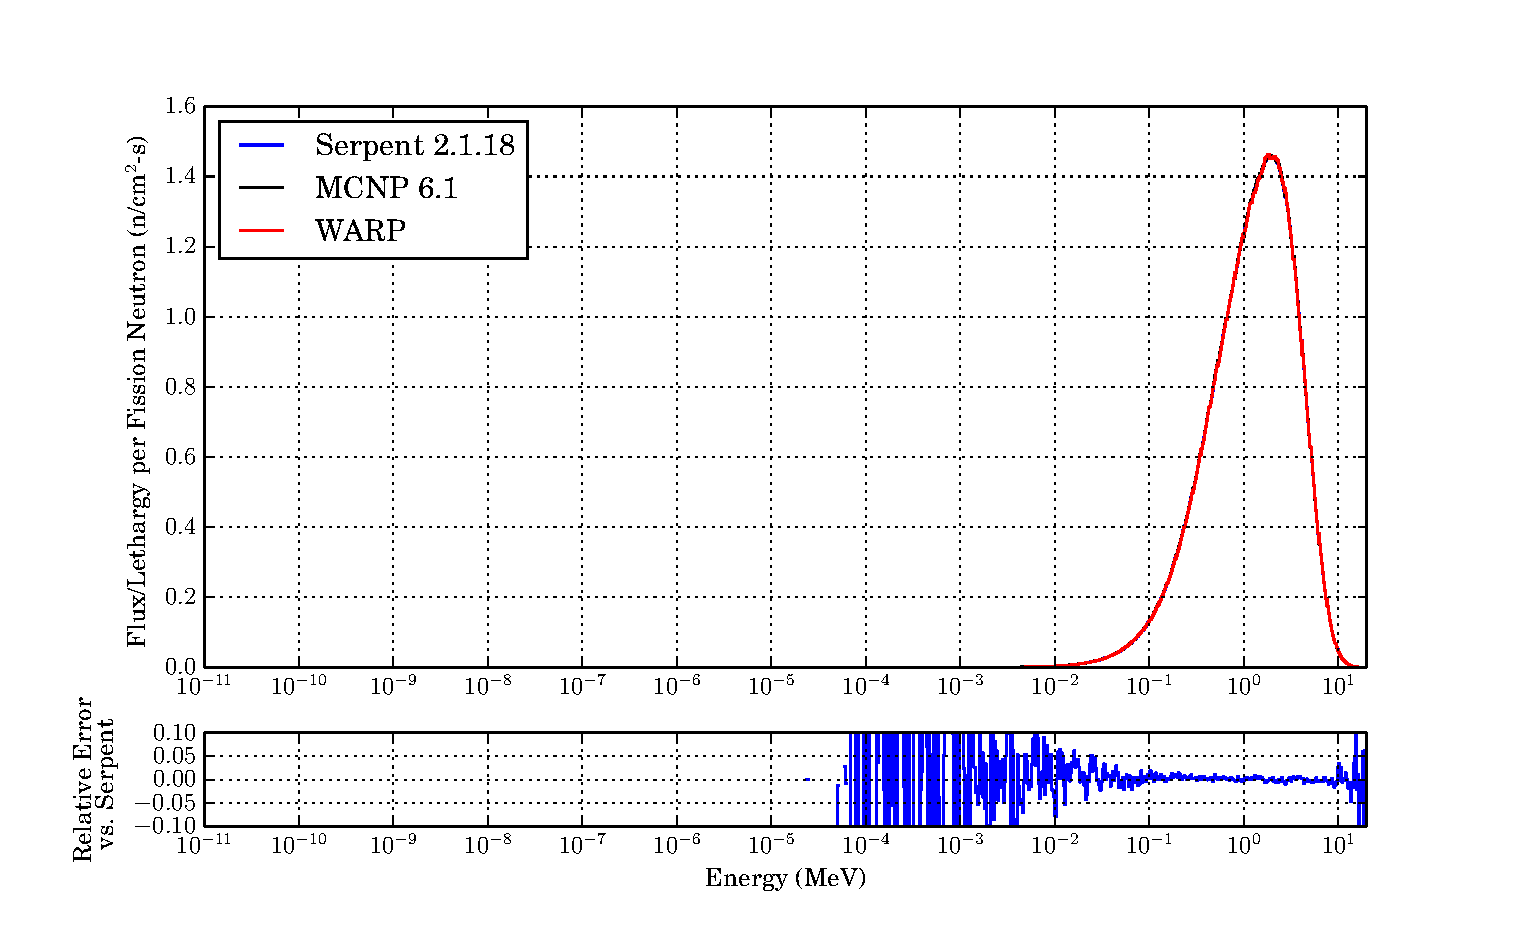
\includegraphics[width=\textwidth]{graphics/finalresults/godiva_spec-6.eps}
\caption{Spectrum comparison in a ``jezebel'' bare pu-239 sphere.. \label{godiva_spec} }
\end{figure}

\begin{figure}[h!]
\centering
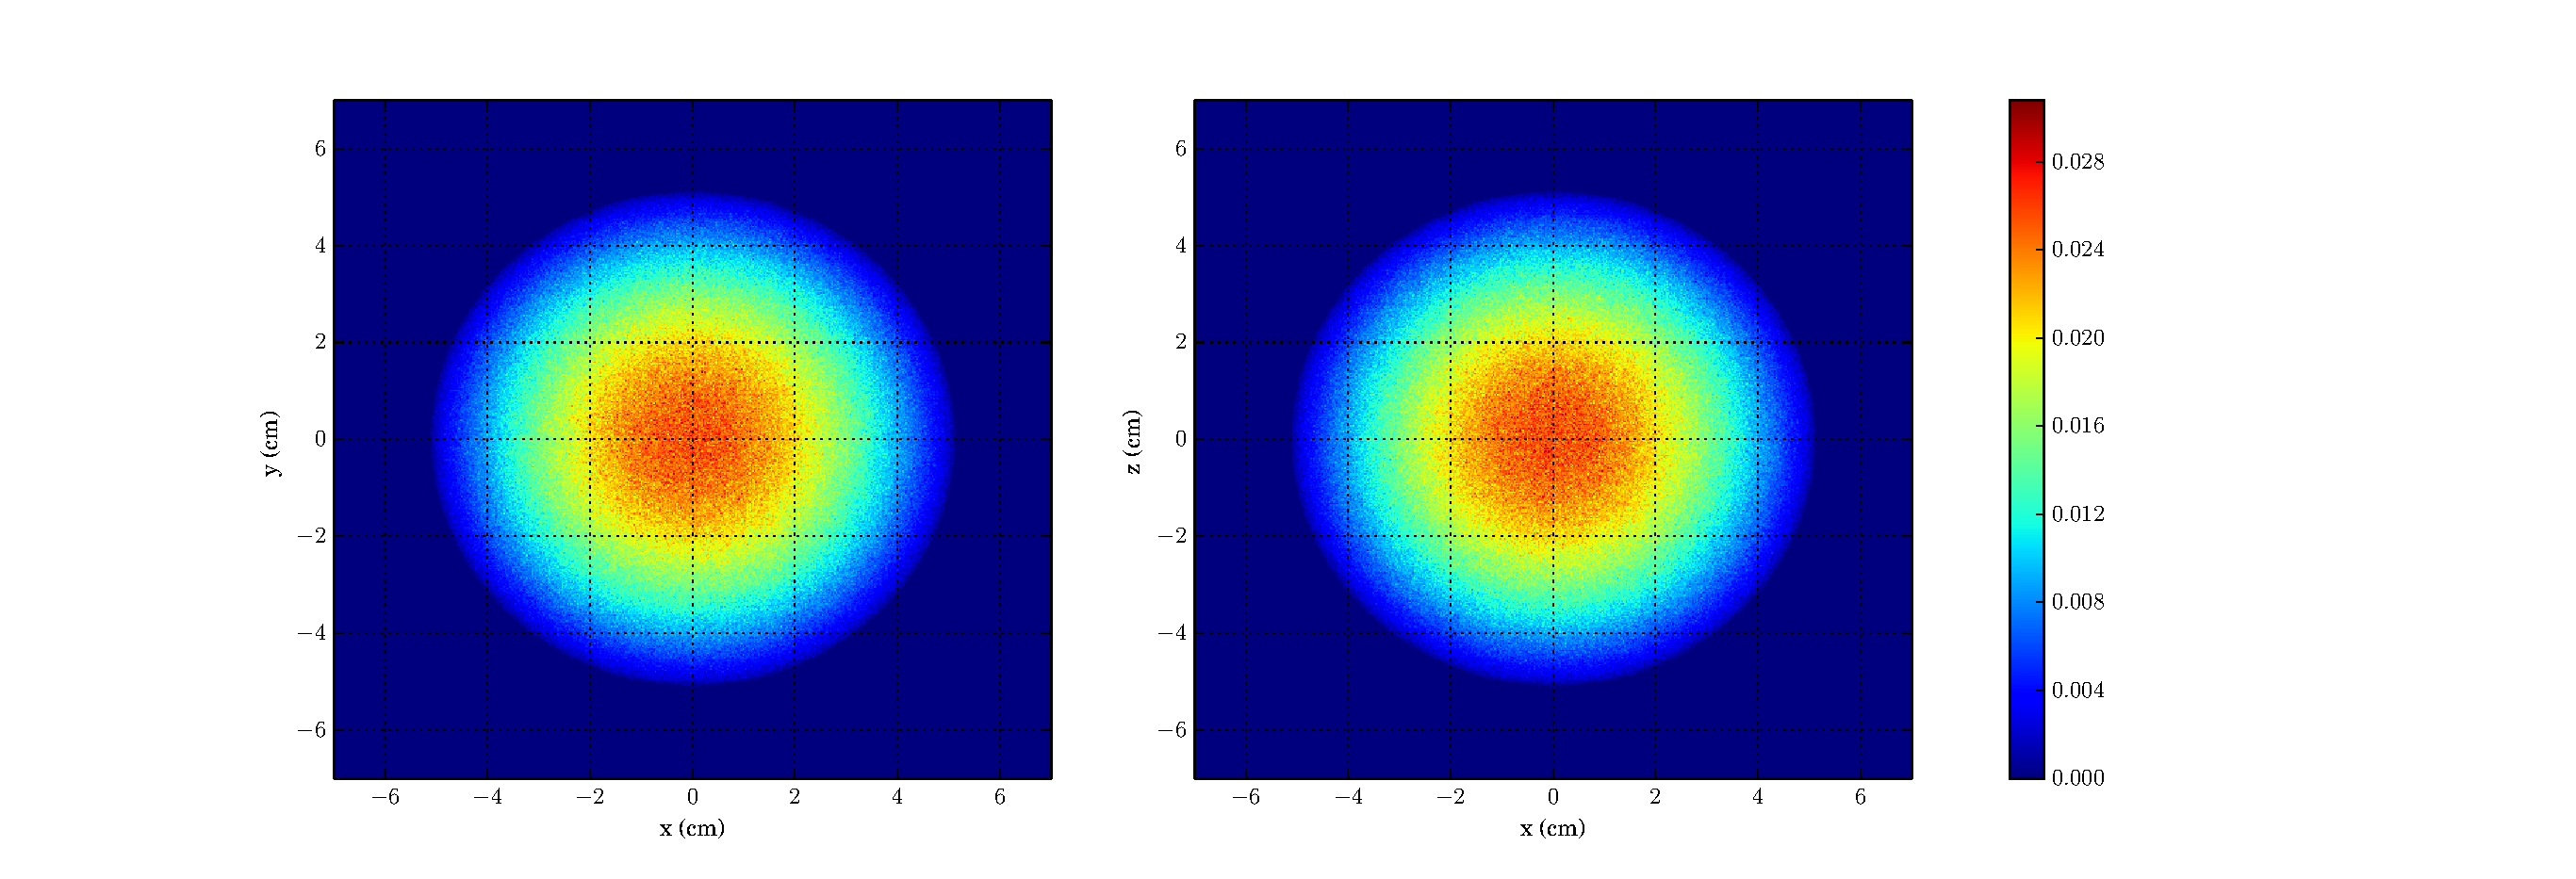
\includegraphics[width=\textwidth,trim= 2cm 0cm 2cm 0cm]{graphics/finalresults/godiva_fiss-6.eps}
\caption{Fission source distribution of a ``jezebel'' bare pu-239 sphere. \label{godiva_fiss} }
\end{figure}

\begin{figure}[h!] 
\centering
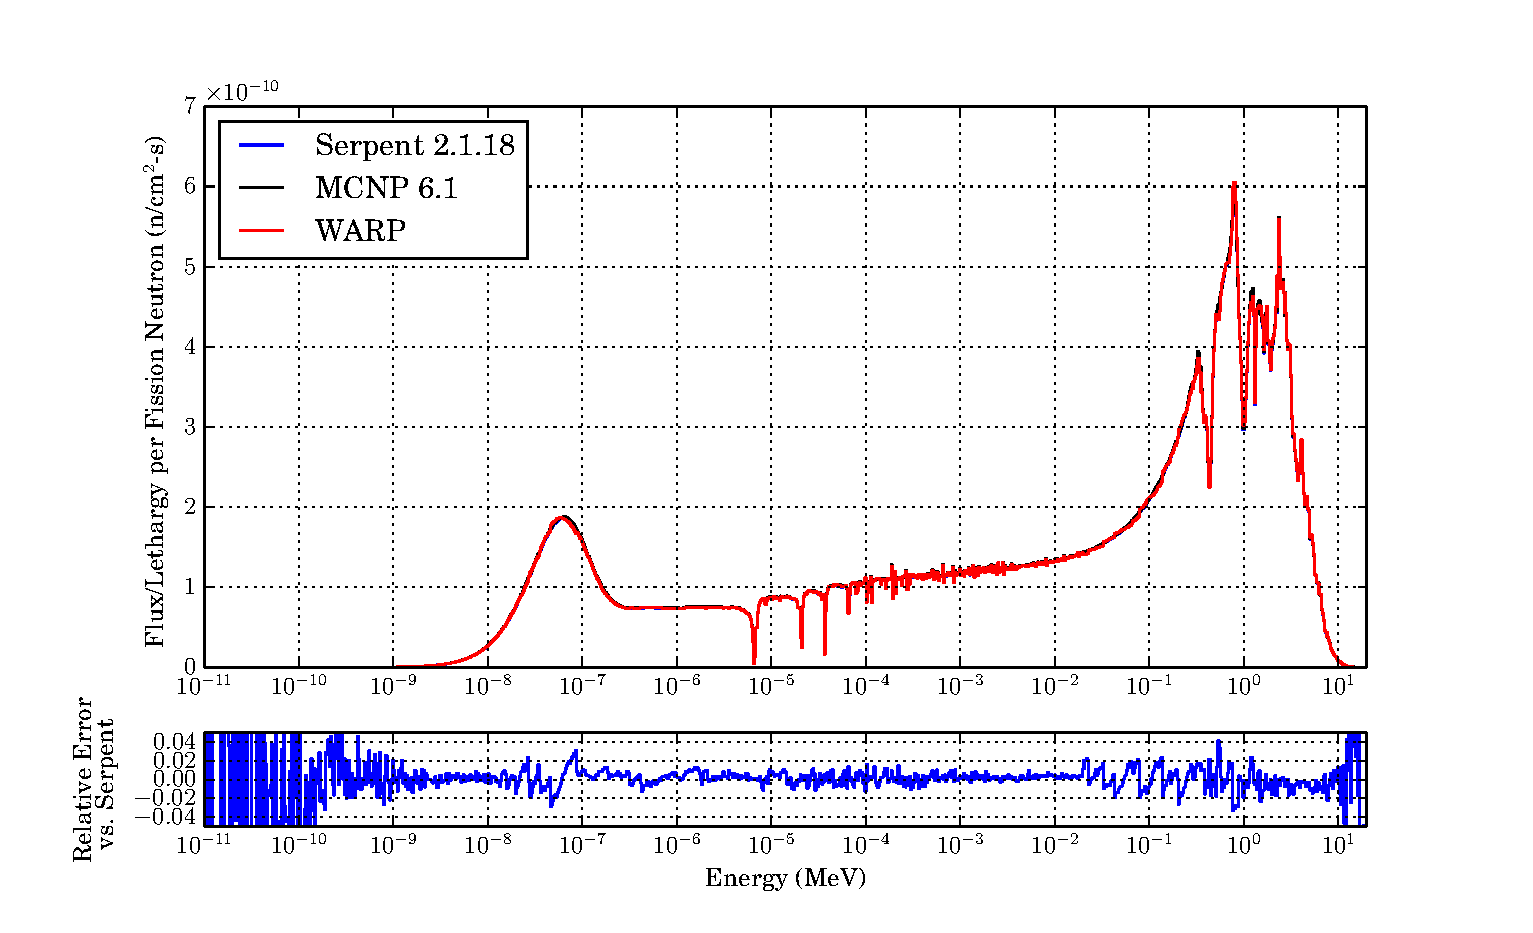
\includegraphics[width=\textwidth]{graphics/finalresults/homfuel_spec-6.eps}
\caption{Spectrum comparison in a homogenized block of UO$_2$ and water. \label{homfuel_spec} }
\end{figure}

\begin{figure}[h!]
\centering
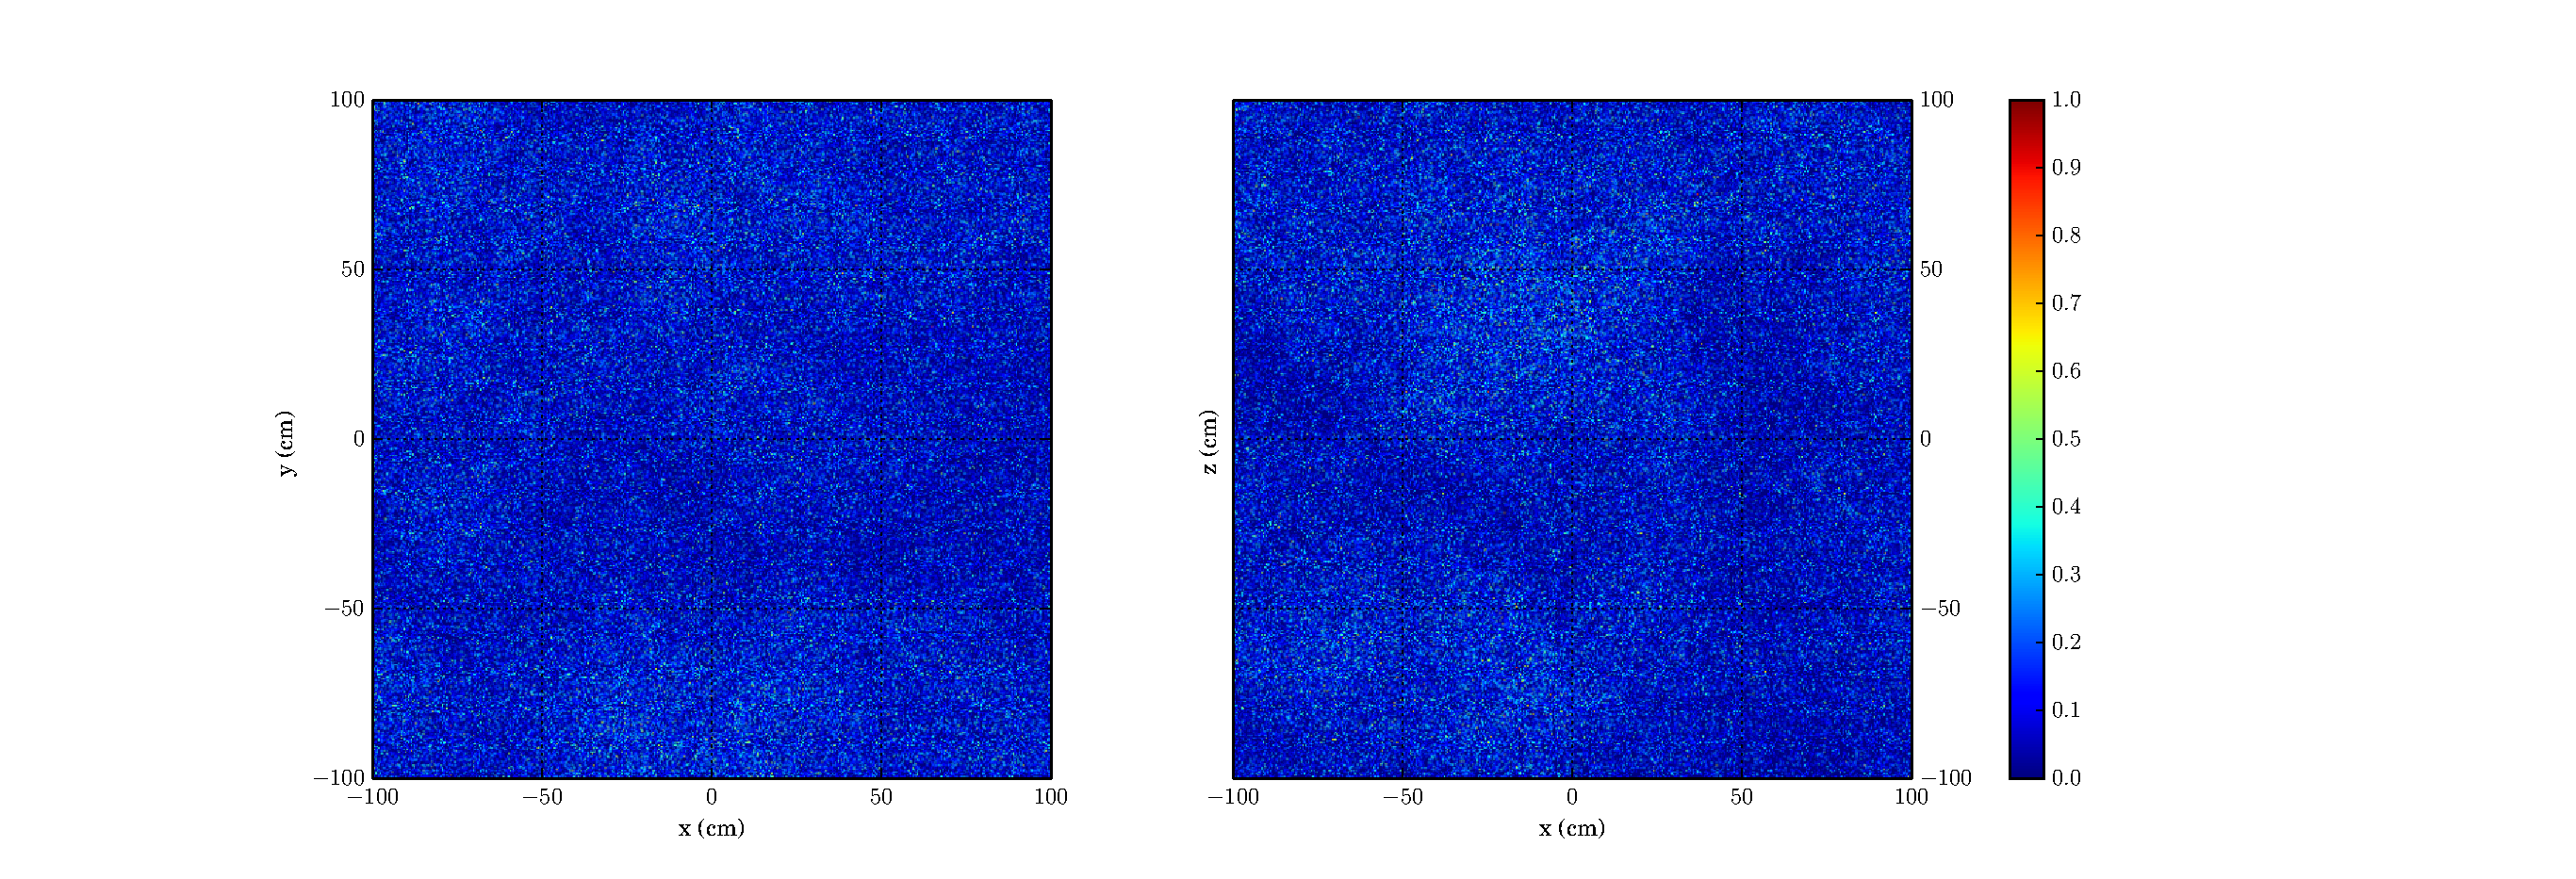
\includegraphics[width=\textwidth,trim= 2cm 0cm 2cm 0cm]{graphics/finalresults/homfuel_fiss-6.eps}
\caption{Fission source distribution of a homogenized block of UO$_2$ and water. \label{homfuel_fiss} }
\end{figure}

\begin{figure}[h!] 
\centering
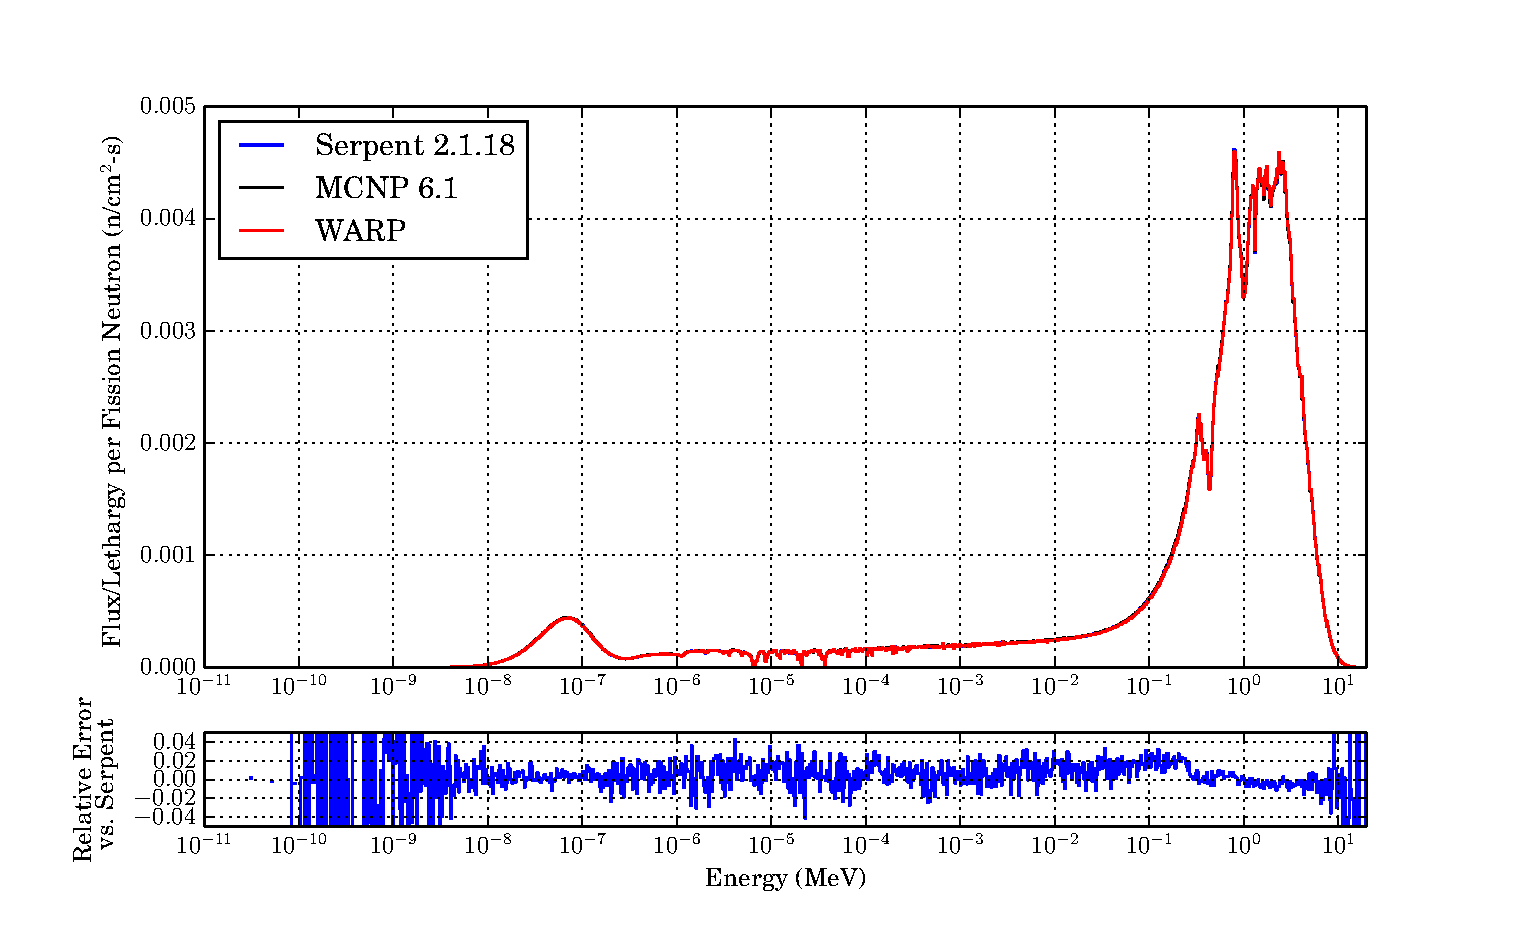
\includegraphics[width=\textwidth]{graphics/finalresults/pincell_spec-6.eps}
\caption{Spectrum comparison in a single UO$_2$ pin surrounded by a block of water. \label{pincell_spec} }
\end{figure}

\begin{figure}[h!]
\centering
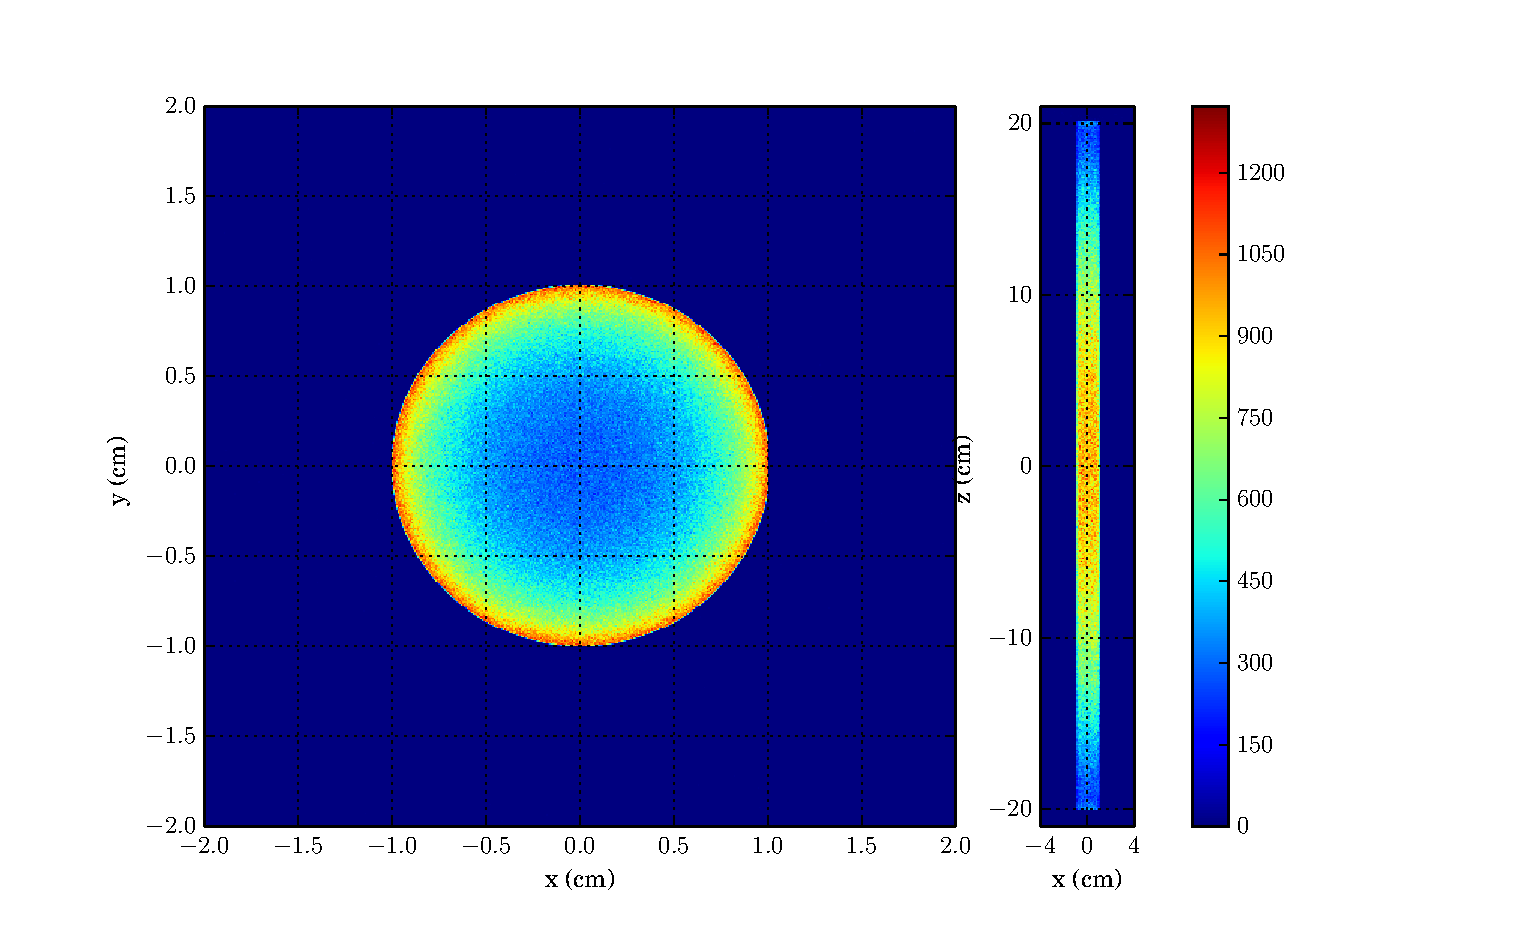
\includegraphics[width=.8\textwidth]{graphics/finalresults/pincell_fiss-6.eps}
\caption{Fission source distribution of a single UO$_2$ pin surrounded by a block of water. \label{pincell_fiss} }
\end{figure}

\begin{figure}[h!] 
\centering
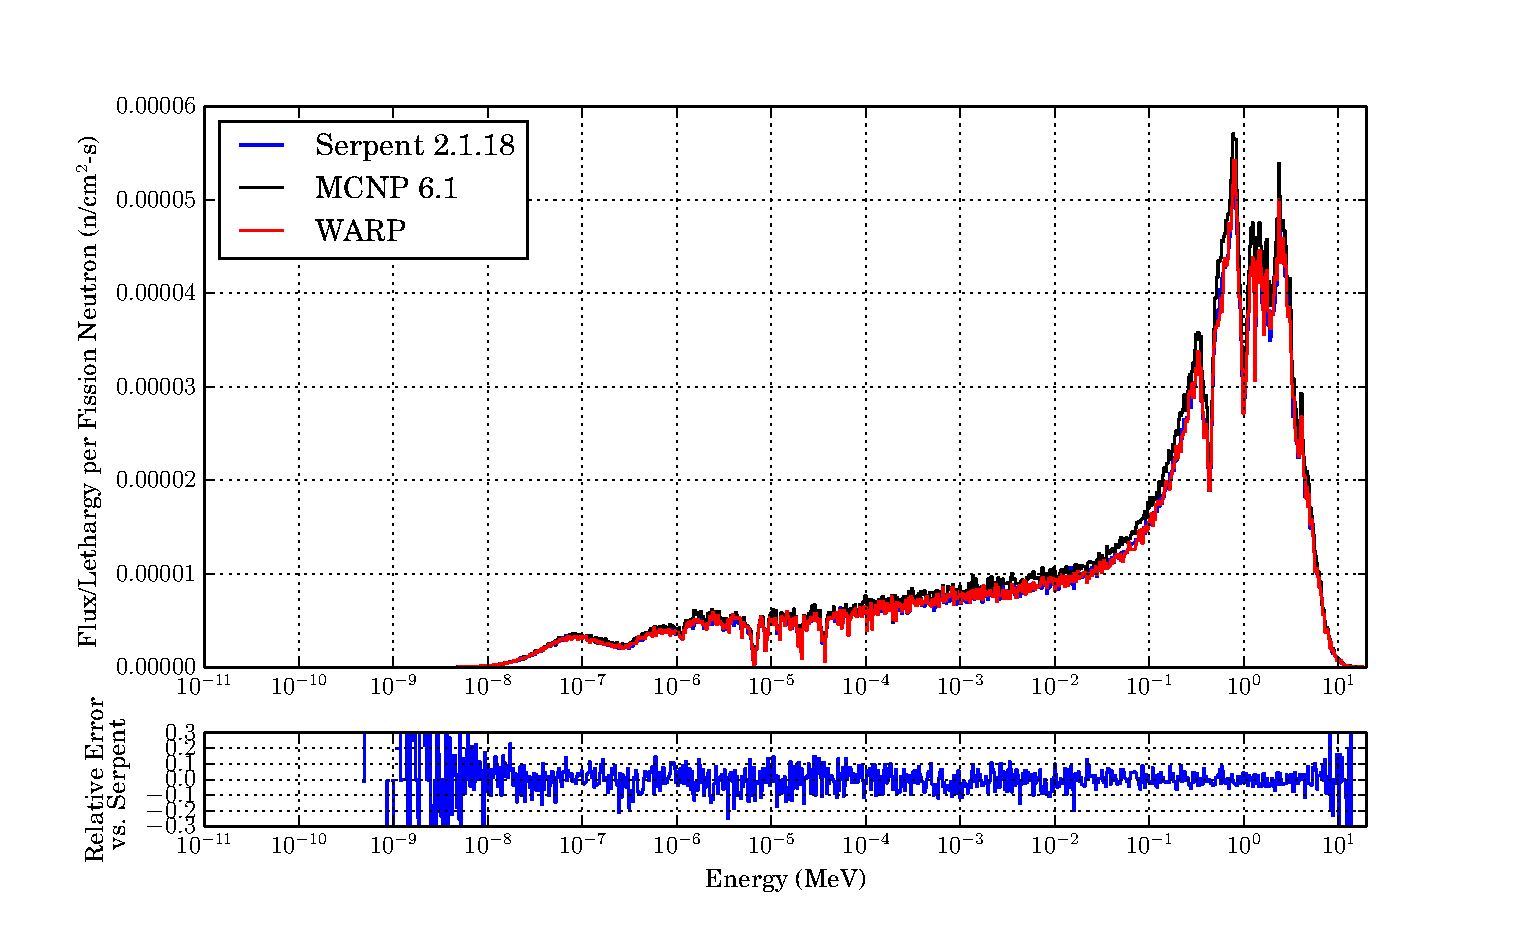
\includegraphics[width=\textwidth]{graphics/finalresults/assembly_spec-6.eps}
\caption{Spectrum comparison in the center UO$_2$ pin of a 15-sided hex pin array in water. \label{assembly_spec} }
\end{figure}

\begin{figure}[h!]
\centering
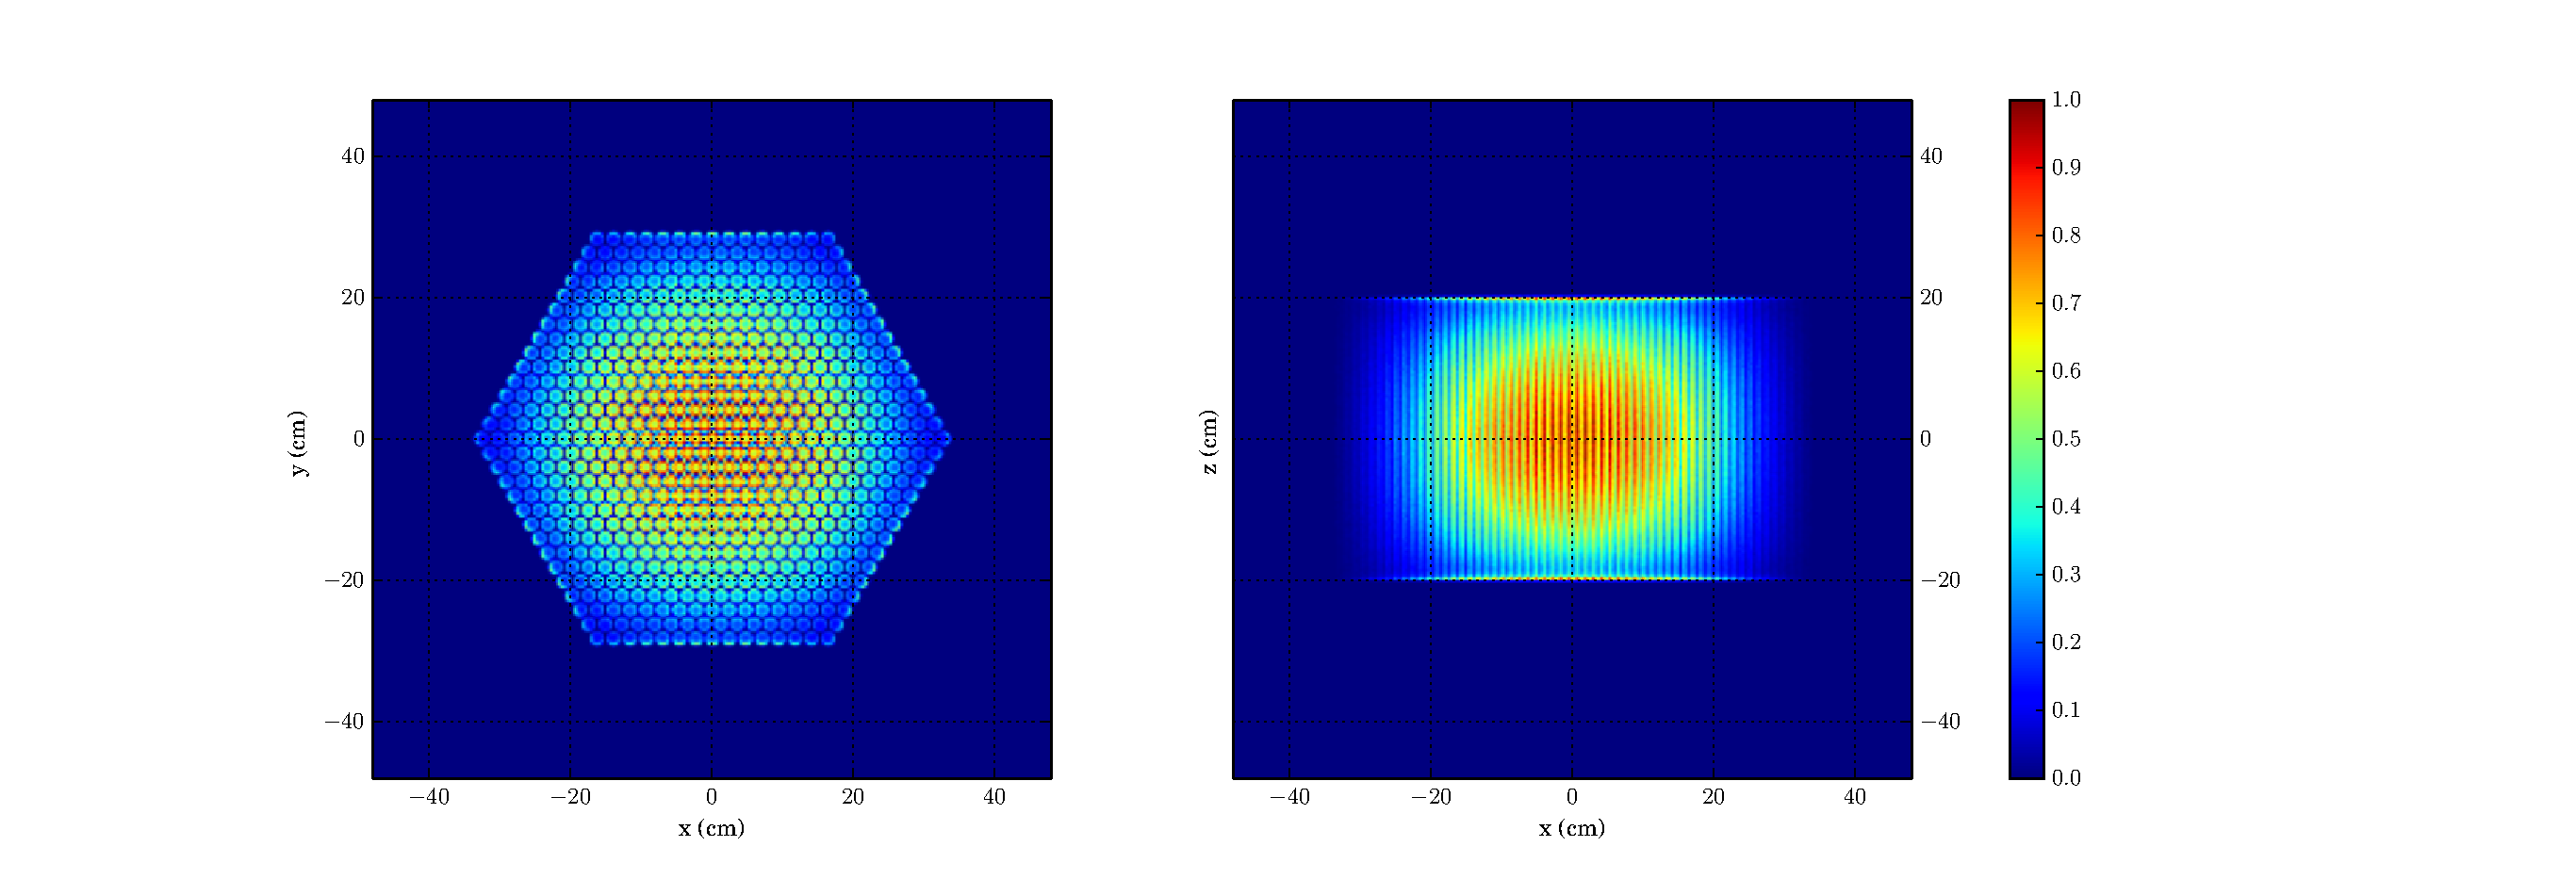
\includegraphics[width=\textwidth,trim= 2cm 0cm 2cm 0cm]{graphics/finalresults/assembly_fiss-6.eps}
\caption{Fission source distribution of an array of UO$_2$ pins in water. \label{assembly_fiss} }
\end{figure}

simple geometry serpent is slow since woodcock makes it sample the geom much more before leaking?, mcnp and warp can instantly leak it?  shouldn't be seen in the homogenized case... yep!

low number not not saturate the gpu, not enough payload for the overhead , pipelining

\section{Fixed Source}'

\begin{table}[h]
\centering
\caption{Summary of $k_\mathrm{eff}$ single-run results of the WARP benchmarks with 20/40 discarded/active criticality cycles and $10^6$ histories per cycle.}
\label{fixed_summary}
\begin{tabular}{| l | r | r | r | r | r |}
 \hline
  U235, 1eV PS & MCNP 6.1 & Serpent 2.1.18 & WARP & $\Delta$ M & $\Delta$ S  \\
\hline
\hline
 $k_\mathrm{eff}$ & 0.6442 (inferred) & 0.749278$\pm$0.000019 & 0.752093 & -10.8\%  & -281.5 pcm   \\
 \hline
 Runtime               & 35.22 m & 4.317 m &  2.0925 m & 16.8x  & 2.1x  \\
 \hline
\end{tabular}
\end{table}

\begin{figure}[h!]
\centering
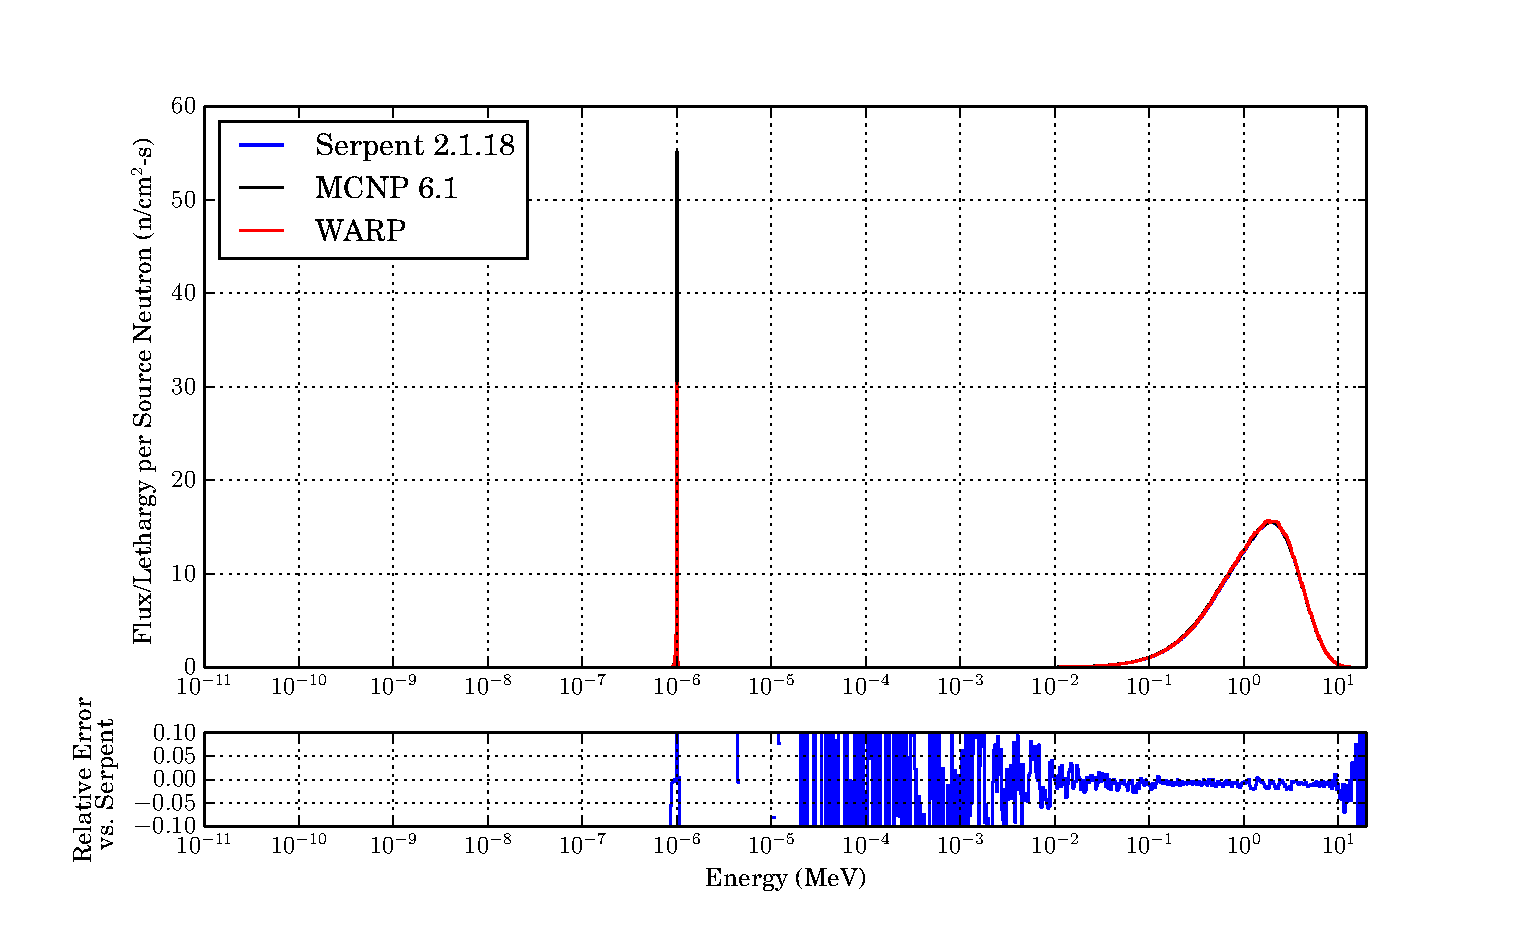
\includegraphics[width=\textwidth]{graphics/finalresults/fixed_spec.eps}
\caption{Flux spectra of fixed source calculations of a 1eV points source in a block of uranium-235 . \label{fixed_spec} }
\end{figure}

fixed source - water slab, accelerator driven subcritical?

\begin{figure}[h!]
\centering
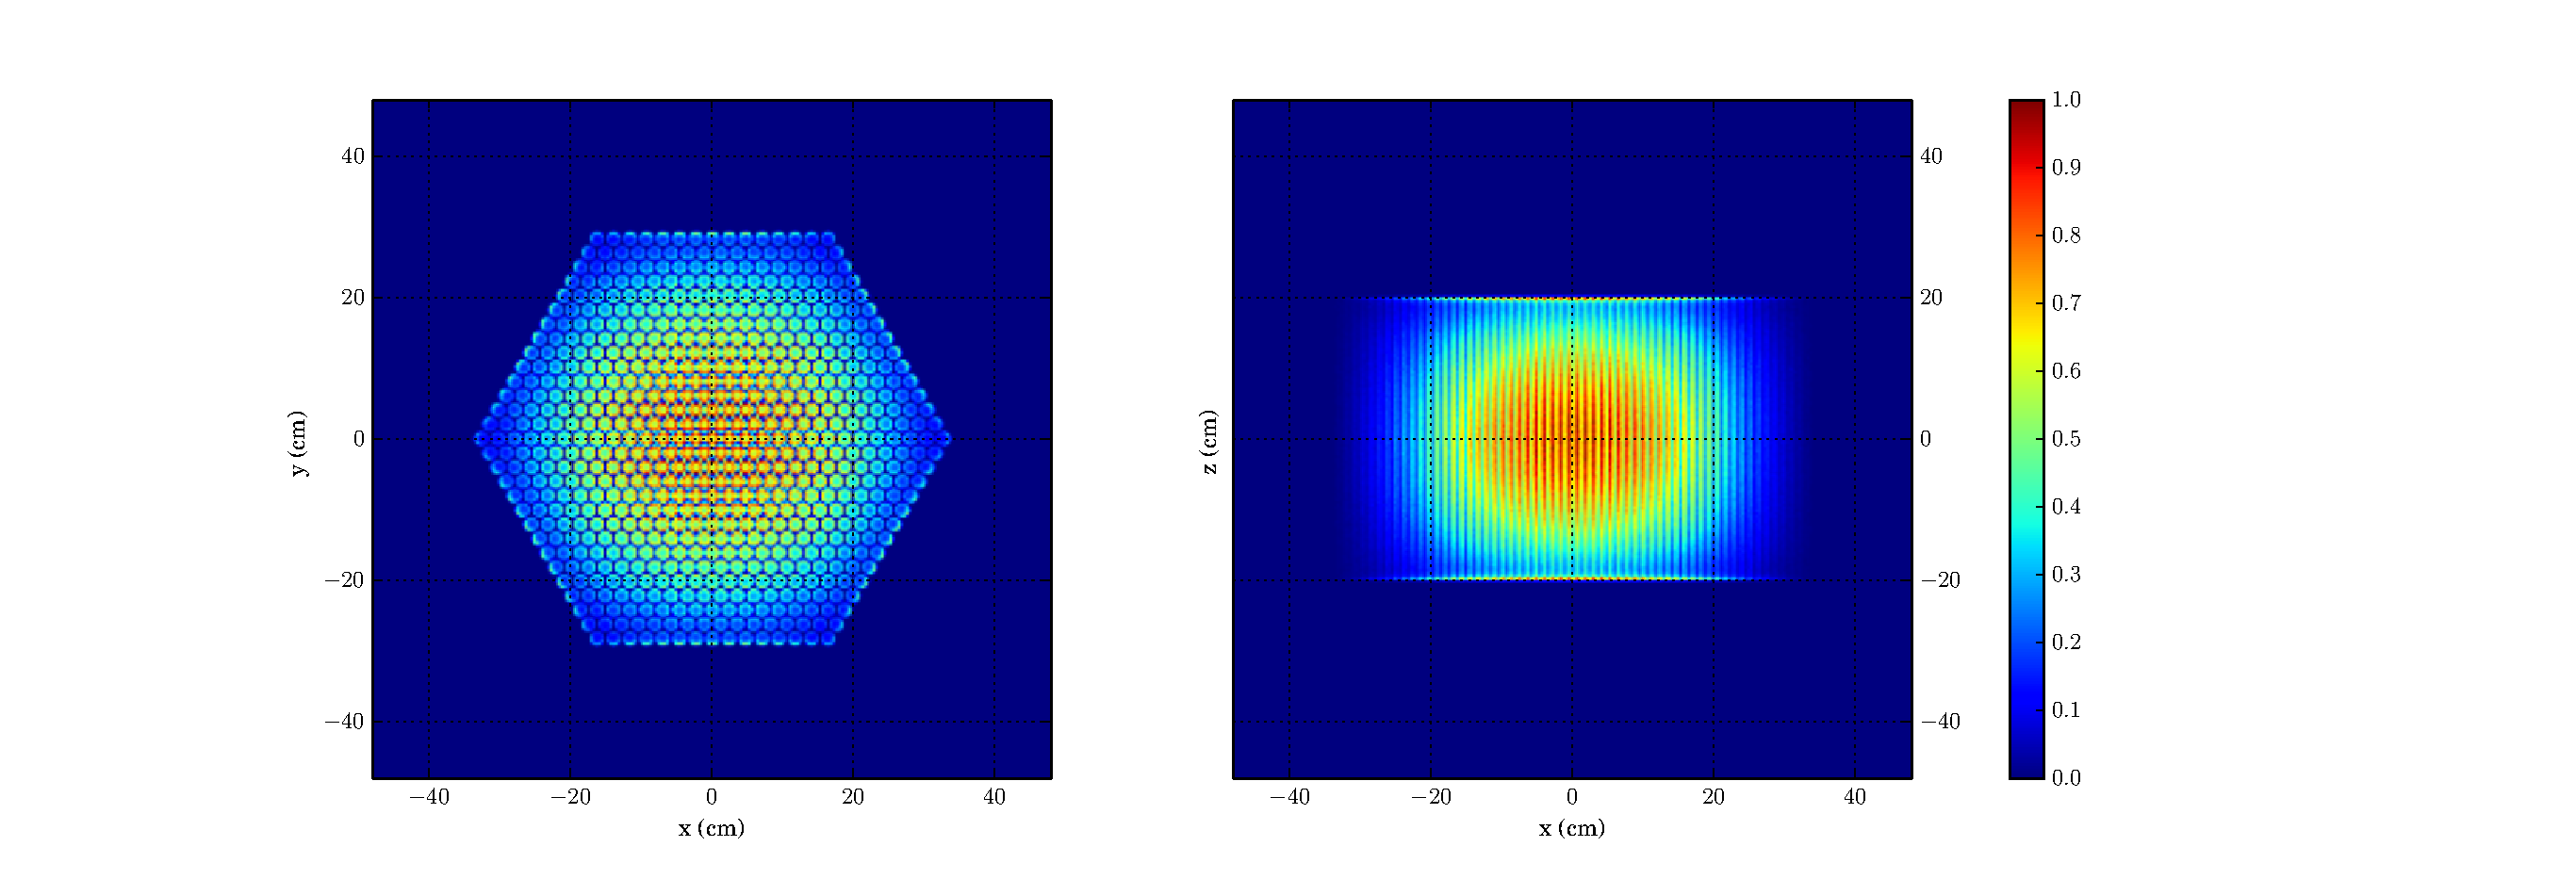
\includegraphics[width=\textwidth,trim= 2cm 0cm 2cm 0cm]{graphics/finalresults/assembly_fiss-6.eps}
\caption{Fission source distribution of an array of UO$_2$ pins in water. \label{assembly_fiss} }
\end{figure}

include?



\section{Run Profiles}

\begin{table}[h]
\centering
\caption{Comparison of the non-remapping and remapping versions of WARP for the four benchmark cases.  20/40 discarded/active criticality cycles and $10^6$ histories per cycle.}
\label{benchmark_nonremapping_summary}
\begin{tabular}{| l | r | r | r |}
 \hline
 Benchmark & Remapping WARP & Non-Remapping WARP & $\Delta k$ or Ratio  \\
\hline
\hline
\multicolumn{4}{|l|}{Jezebel}  \\
\hline
 $k_\mathrm{eff}$ & 1.0279 & 1.0279  & 0 pcm\\
 \hline
 Runtime               &   2.0147 m & 1.84 m & 0.91 \\
 \hline
 \hline
\multicolumn{4}{|l|}{Homogenized Block }\\
\hline
 $k_\mathrm{eff}$ & 0.9426 & 0.941857 & 74.3 pcm  \\
 \hline
 Runtime               &  3.934 m & 4.05 m & 1.03 \\
 \hline
  \hline
\multicolumn{4}{|l|}{Pin Cell}\\
\hline
 $k_\mathrm{eff}$ &  0.3804 & 0.38063  & -23 pcm \\
 \hline
 Runtime               & 7.0682 m & 10.52 m & 1.49 \\
 \hline
  \hline
\multicolumn{4}{|l|}{15-sided Hex Assembly}\\
\hline
 $k_\mathrm{eff}$  & 1.4454  & 1.4457 & -30 pcm \\
 \hline
 Runtime               & 7.9703 m & 95.85 m & 12.03 \\
 \hline
\end{tabular}
\end{table}

\begin{table}[h]
\centering
\caption{Summary table of the time spent in each WARP subroutine in criticality mode for each benchmark case.}
\label{profile_summary}
\begin{tabular}{| l | r  | r | r | r |}
\multicolumn{5}{l}{Remapping} \\
 \hline
 Subroutine & Jezebel & Homogenized Block & Pincell & 15-sided Hex Assembly  \\
\hline
\hline
\multicolumn{5}{l}{} \\
\multicolumn{5}{l}{Non-Remapping} \\
 \hline
 Subroutine & Jezebel & Homogenized Block & Pincell & 15-sided Hex Assembly  \\
\hline
\hline
\end{tabular}
\end{table}

\begin{figure}[h!]
\centering
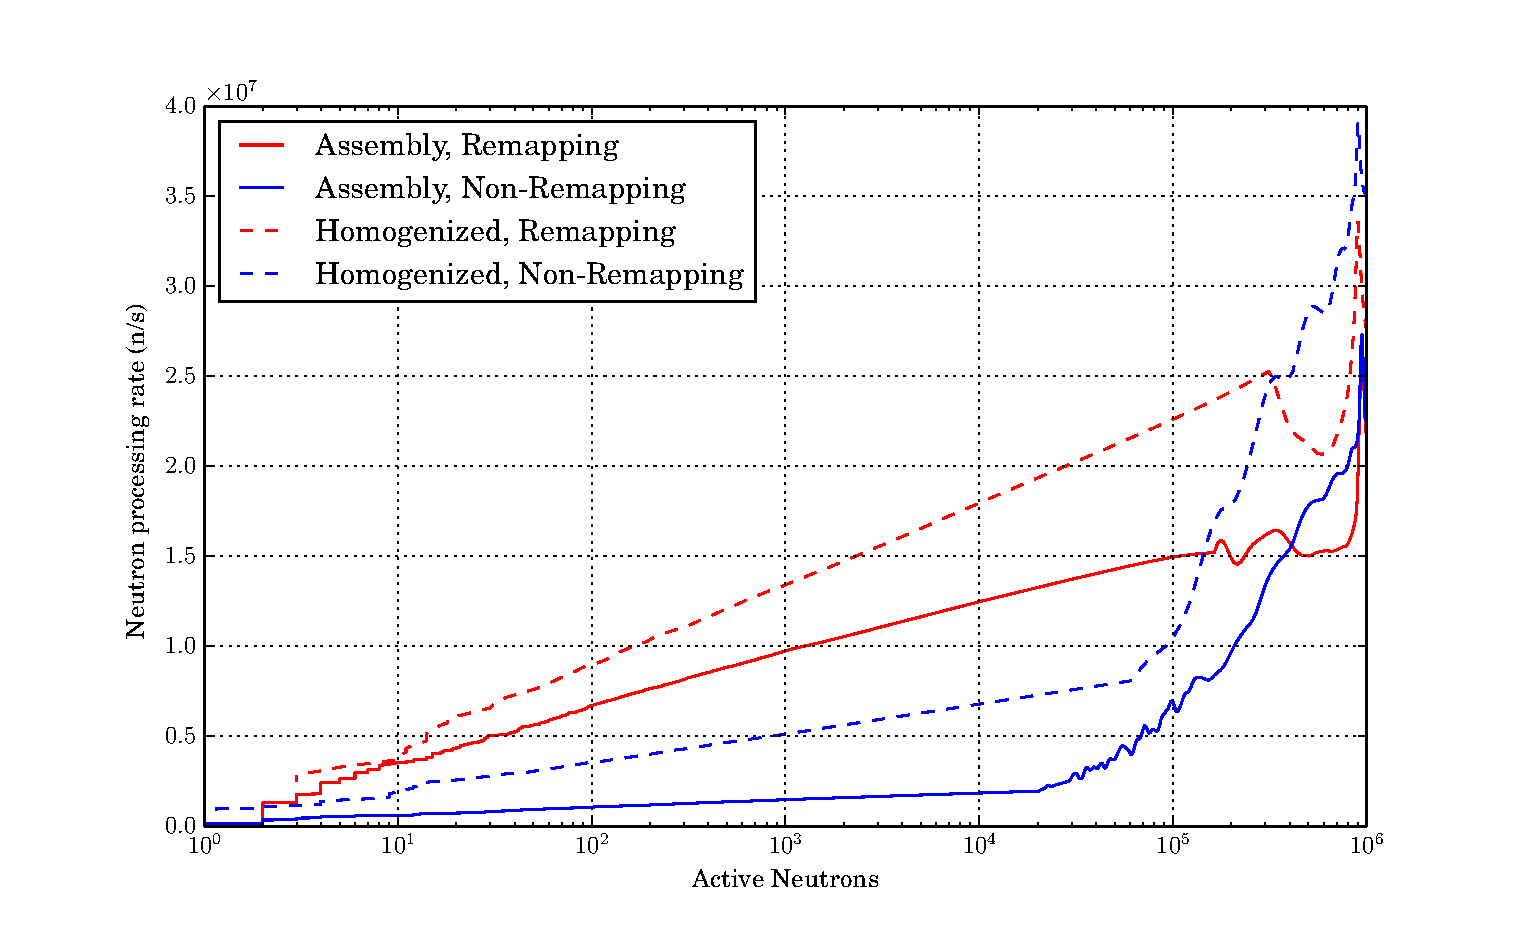
\includegraphics[width=\textwidth]{graphics/finalresults/process_rate.eps}
\caption{Neutron processing rate of WARP in the homogenized block and assembly benchmark cases. \label{process_rate} }
\end{figure}

profiler stuff, time in each routine.  compare assembly and homfuel.  compare w non-remapped

stats, the way the active particles die off for assembly and homfuel.  include the non-remapped version in the time/cycle plot.  runtimes...

remapping has a HUGE impact on OptiX runtime.




